\section{2D TMD Heterojunction Gas Sensors}
\label{sec:2d_tmd_heterojunction_gas_sensors}
%\note{Two 2D TMD heterojunction gas sensors \cite{Kim2020, Liu2021} shall be presented in detail. Their differences in fabrication/performance/scaleability/etc. shall be analyzed. They shall also be compared to conventional gas sensors. Problems that hinder a large scale production shall be identified and possible solution attempts shall be presented.}

As has been stated earlier in this publication, \gls{tmd} gas sensor are very promising in regards to being the next generation of gas sensors. However, their large scale application has yet to be seen. This section shall identify why this is not yet the case. To do that, two gas sensors and their design philosophies shall be shown in detail. Their performance, longevity, scalebality and potential for mass fabrication shall be analyzed and shall be compared to conventional gas sensors.  \\
The first sensor (Sensor 1) is the one proposed by \cite{Kim2020}. It is based on a WSe2/WS2  heterojunction. The WSe2 film has been exposed to the environment. As it exhibits p-type semiconductor properties, it is especially sensitive to the electron accepting NO2 gas. As explained in \Cref{sec:functionality}, one advantage of heterojunction based gas sensors is the increased sensitivity to gas adsorption. The proposed sensor exhibits another favorable property: A photovoltaic effect. When light of the intensity of \SI{10}{\watt\per\meter^2} is shone onto the sensor, a short circuit current of \SI{0.9}{\milli\ampere} is measurable. This effect implies, that the sensor does not have to be supplied with external power and that the current, induced by the photovoltaic effect, can be utilized as measurement signal. The layer thickness of both materials was part of a compromise between the magnitude of the photovoltaic effect, and the revovery time of the sensor. A greater layer thickness would increase the photovoltaic effect however, the recovery time of the sensor at room temperature would have been increased. It has been decided to fabricate the sensor with three layers of WSe2 and WS2 respectivelly, resulting in an overall thickness of \SI{4.5}{\nano\meter} (excluding the substrate). The topology of the device has been inspected via Raman spectroscopy, \gls{tem}, \gls{afm} and \gls{eds}. \\
The second sensor (Sensor 2), that shall be discussed, has been fabricated by \cite{Liu2021}. Its strategy is to intentionally pollute MoS2 nanosheets with ZnS in order to generate lots of hetrojunctions, dotted around the surface of the sensor. These impurity sites, for once, create small space charge regions, which modulate the conductivity of the material. Additionally to that, these sites provide docking sites for the analyte gas. This effectivelly increases the adsorption rate of the sensor and thus increases its sensitivity. The sensor does not have photovolotaic properties. The Measurement principle is therefore purely resistive. The surface morphology of the film has been verified via Raman spectroscopy and \gls{tem}.\\
\subsection{Sensing Performance}
The sensing performance of a gas sensor is usually quantified by its response value $S$. This value is a ratio of its primary measurement parameter in a clean environment and within an environment with specific gas concentration. \Cref{eqn:respone_1,eqn:respone_2} shows the most common definitions of the response metric. $\bullet_a$ refers to the measurement value in an environment without the analyte gas. $\bullet_g$ is the measurment value in an environement with a specific concentration of the analyte gas. $R$ refers to a resistance value, while $I$ identifies an electric current.
\begin{equation}
\label{eqn:respone_1}
    S = |\frac{R_g-R_a}{R_a}|
\end{equation}
\begin{equation}
\label{eqn:respone_2}
    S = |\frac{I_g-I_a}{I_a}|
\end{equation}

As Sensor 1 relies on current measurement and Sensor 2 on modulation of the conductivity, the response definition from \Cref{eqn:respone_1} and \Cref{eqn:respone_2} shall be used respectivelly. \\ 
Closely related to the response metric of a gas sensor is the lower detection limit $c_{min}$. It specifies the lowest anaylte gas concentration the sensor is able to detect. It is mainly determined by the response and background noise of the sensor. The U.S. Environmental Protection Agency recommends an exposure limit to NO2 of \SI{53}{ppb}. Ideally, the detection limit of gas sensors should be below that value. \\
Another important characteristics are the response time $t_{resp}$ and the recovery time $t_{rec}$. They define how fast the sensor reacts to changes in gas concentration and how fast the sensor recovers to its initial state, after the environment has been purged of the analyte gas. Usually both times are measured by subjecting the sensor to a specific analyte gas concentration and then purging the sensor with an inert gas (e.g. N2). The response time $t_{resp}$ is the time span that elapses, until \SI{90}{\percent} of the final measurement value have been reached. Consequently, the recovery time $t_{rec}$ is the time span that elapses, until the sensor response changes by \SI{90}{\percent} after a full exposition and subsequent purging.   \\
\\
Sensor 1 has an response of 1.8 at a NO2 concentration of \SI{10}{ppm} NO2. Sensor 2 shows a response of 8.1 at the same concentration. The detection limit lies at \SI{14}{ppb} for Sensor 2. Sensor 1 did not provide a value here. Both sensors have been evaluated at room temperature (\SI{25}{\celsius}). The response time has been measured to be \SI{6}{\minute} and \SI{1}{\minute} respectivelly.  Recovery times have been determined to be \SI{12}{\minute} and \SI{4.6}{\minute} respectivelly. \Cref{tab:comparison} gives an overview of this comparison.\\
It can be seen, that Sensor 2 exposes superior measures in every way. Especially the low detection limit and high response values are outstanding. The performance of Sensor 1 is still mentionable, as no external bias voltage has been applied to it. The whole measurement effect was powered by a \SI{10}{\watt\per\meter^2} white light. As such, it has potential in being implemented in systems, where energy is very scarce.
\begin{table}[]
\centering
\begin{tabular}{lcc}
                    & Sensor 1 & Sensor 2 \\
                    \hline \hline
Response &   1.8 @ \SI{10}{ppm}        &   8.1 @ \SI{10}{ppm}       \\
\hline
Detection Limit    &    N/A      &   \SI{14}{ppb}       \\
\hline
Response Time       &      \SI{6}{\minute}   &  \SI{1}{\minute}        \\
\hline
Recovery Time       &      \SI{12}{\minute}   &  \SI{4.6}{\minute}        \\
\hline
Stability           &      N/A    &   At least \SI{1}{week}       \\
\hline
Working Temperature &      \SI{25}{\celsius}    &  \SI{25}{\celsius} \\
\hline \hline
\end{tabular}
\caption{Comparison between the two presented sensors. All values correspond to NO2 as analyte gas.}
\label{tab:comparison}
\end{table}
\subsection{Fabrication}
Sensor 1 is fabricated by an 6 step process. Starting point is a \Gls{soi} wafer, which has been cleaned with acetone, \gls{ipa} and deionized water.  The WS2 film was deposited by reacting tungsten hexachloride (WCl6) and hydrogen sulfide (H7S) in a \gls{cvd} process. In the same process , WCl6 and Diethylselenide (DESe) has been combined to WSe2. A second substrate has been prepared, where the gold bottom electrode has been prepared. The WS2/WSe2 structure has been transferred onto the gold electrode. Eventually, the palladium top electrode has been patterned onto the WS2/WSe2 structure. \Cref{fig:fabrication_sensor1} depicts the \gls{cvd} portion of the process.\\
The fabrication of Sensor 2 starts with the synthesis of the MoS2 nano sheets. For that, a grinding-assisted liquid-phase exfoliation method was used. This method included grinding, solvation, vigorous sonication and multiple centrifucation steps that have to be applied to MoS2 powders. The nanosheets could be obtained from the precipitants of that process. The \enquote{pollution} with ZnS has been achieved by mixing the MoS2 nanosheets with Zn(CH3COO)2*2H2O and Na2S*9H20 while being dissolved in deionized water. An interdigitated electrode pair, consisting of Au and Ti, has been prepared on \gls{soi}. The prepared MoS2/ZnS solution has then been furhter dilluted with ethanol and subsequently been dripped onto the electrode structure. After a drying step, the MoS2/ZnS structure was finished. The final step consisted of a transfer of the \gls{soi} chip onto a copper substrate for better connectivity.
\begin{figure}
\centering
\begin{subfigure}{\textwidth}
    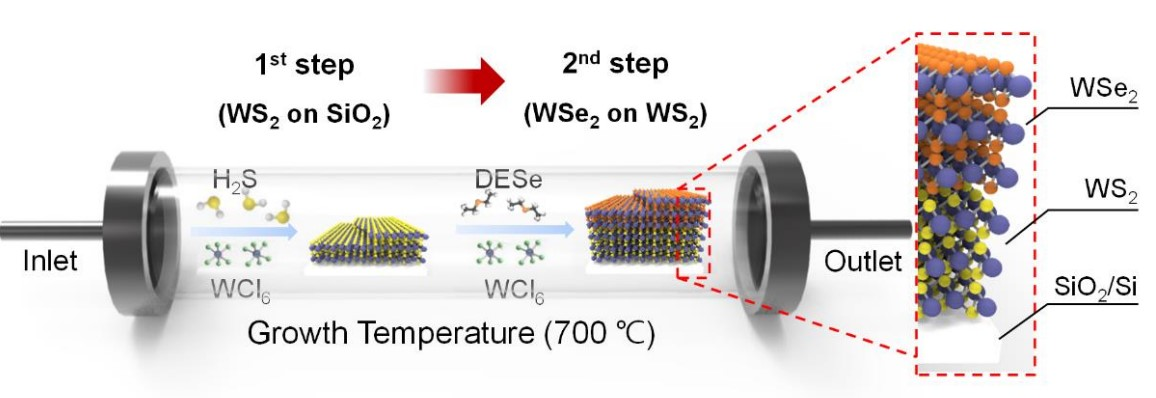
\includegraphics[width=\textwidth]{04_2d_tmd_heterojunction_gas_sensors//fig/sensor1_fabrication.jpg}
    \caption{}
    \label{fig:fabrication_sensor1}
\end{subfigure}
\begin{subfigure}{\textwidth}
    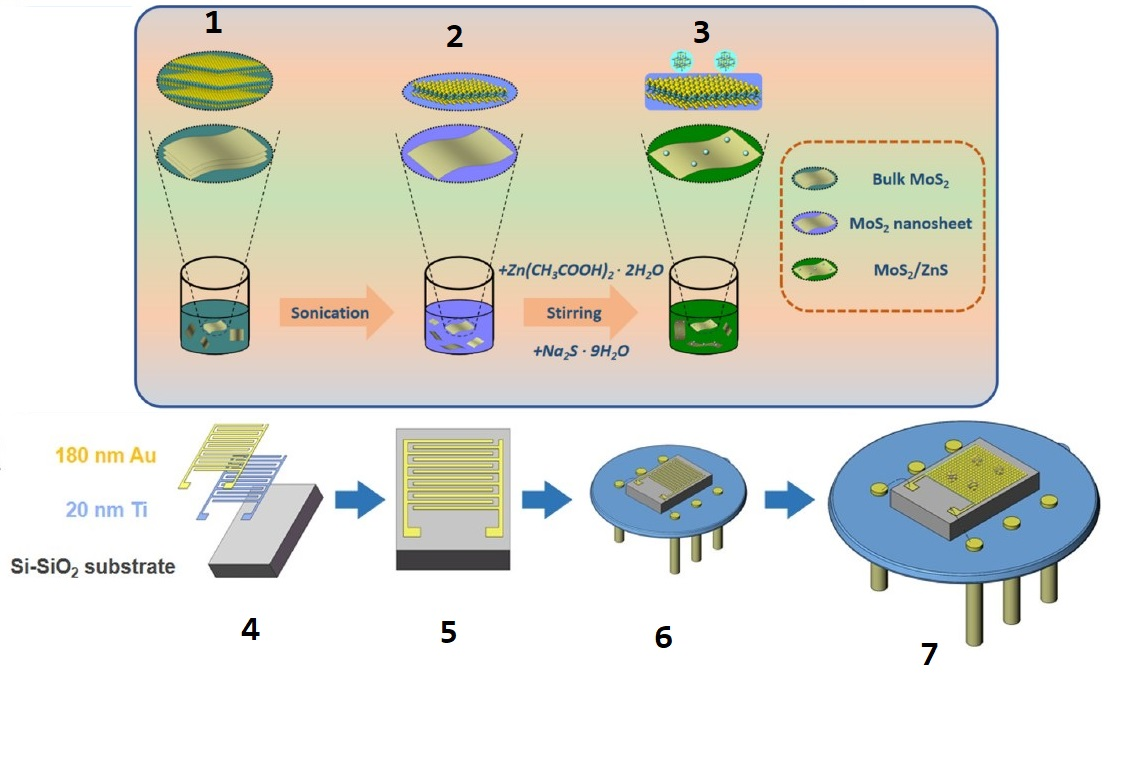
\includegraphics[width=\textwidth]{04_2d_tmd_heterojunction_gas_sensors//fig/sensor2_fabrication.jpg}
    \caption{}
    \label{fig:fabrication_sensor2}
\end{subfigure}
\caption{The fabrication processes of Sensor 1 (\cref{fig:fabrication_sensor1}) and Sensor 2 \cref{fig:fabrication_sensor2}.}
\label{fig:fabrication}
\end{figure}
\subsection{Scalability}
One of the most important factors that determines the scalability and hence the mass producability of semi conductor devices, is the complexity of their fabrication. With the complexity mostly originating from the count the different fabrication methods being used. Another criteria for good scalability is the compatibility to the \gls{cmos} fabrication process. This property enables the fabrication of the target device on the same wafer as \glspl{mosfet} will be fabricated. This enables the integrated fabrication of sensing device, analog frontend and digital processing without the need of costly and time consuming transfer processes. Due to its outstanding advantages with regards to footprint size and reduced manufacturing cost, it is a quality that is highly sought after.\\
Fabrication of sensor 1 consists of six steps which are mainly executable within a \gls{cvd} chamber. A single transfer process is necessary, in order to transport the 2D material onto the contact electrodes. Apart from the transfer step, the process is simple and shows potential for scaling. Compaitiblity to \gls{cmos} processes has to be judged on a per-case basis, as a temperature of \SI{700}{\celsius} is necessary, during the film synthesis. This temperature could reactivate the diffusion in some doped regions and therefore could be detrimental to the integration into \gls{cmos} processes.\\
Sensor 2 fabrication is concluded after seven steps. Although, the transfer process uses \gls{dep}, and as such could have potential to be scalable, the fabrication of the nanosheets and the application of the nano dots, is a highly manual process, which seems to be hardly automatable. As no high temperature processes are needed, \gls{cmos} compatibility is given. The only challenge is to introduce the dissolved nanoparticles into the fabrication line.
\subsection{Stability}
The stability (or life span) specifies the period of time, the sensor adheres to its specification. a high stability decreases the rate at which sensors have to be replaced. Usually the readout of the sensors is also simplified, as fewer drift compensation has to be considered. The life span of a sensor is highly dependent on its environment. For instance, the commercially available NO2 sensor FECS42-20 specifies a life span of over two years \cite{Figaro}. \\ 
Sensor 1 did not provide any measures on long term drift of the sensor parameters. There seem to be no other publications with identical layer stack configuration. The closest device, sensor 1 could compare to, is the one presented in \cite{Wu2020} as both sensors expose a WSe2 surface to the environment. There, no significant degradation has been noticed, within the test period of 60 days. \\
An evaluation of the long term stability of sensor 2 has been done. The response metric dropped from 7.3 to 7.1 within one week and seemed to stabilize there.
